\documentclass{article}

\usepackage{PRIMEarxiv}

\usepackage[utf8]{inputenc} % allow utf-8 input
\usepackage[T1]{fontenc}    % use 8-bit T1 fonts
\usepackage{hyperref}       % hyperlinks
\usepackage{url}            % simple URL typesetting
\usepackage{booktabs}       % professional-quality tables
\usepackage{amsfonts,amsmath}       % blackboard math symbols
\usepackage{nicefrac}       % compact symbols for 1/2, etc.
\usepackage{microtype}      % microtypography
\usepackage{lipsum}
\usepackage{fancyhdr}       % header
\usepackage{graphicx}       % graphics
\usepackage{subcaption}
\graphicspath{{media/}}     % organize your images and other figures under media/ folder

%Header
\pagestyle{fancy}
\thispagestyle{empty}
\rhead{ \textit{ }} 

% Update your Headers here
\fancyhead[LO]{Far-field potential flow conditions for Immersed Cartesian meshes}
% \fancyhead[RE]{Firstauthor and Secondauthor} % Firstauthor et al. if more than 2 - must use \documentclass[twoside]{article}



  
%% Title
\title{Far-field potential flow conditions for Immersed Cartesian meshes
%%%% Cite as
%%%% Update your official citation here when published 
\thanks{\textit{\underline{Citation}}: 
\textbf{Authors. Title. Pages.... DOI:000000/11111.}} 
}

\author{
    Gabriel D. Weymouth\\
    Ship Hydromechanics\\
    Mechanical, Maritime and Material Engineering Departement (3mE) \\
    Delft University of Technology, Delft, Netherlands \\
    \texttt{G.D.Weymouth@tudelft.nl} \\
    \AND
    Marin Lauber\\
    Ship Hydromechanics\\
    Mechanical, Maritime and Material Engineering Departement (3mE) \\
    Delft University of Technology, Delft, Netherlands \\
    \texttt{marinlauber@tudelft.nl} \\
  %% \AND
  %% Coauthor \\
  %% Affiliation \\
  %% Address \\
  %% \texttt{email} \\
  %% \And
  %% Coauthor \\
  %% Affiliation \\
  %% Address \\
  %% \texttt{email} \\
  %% \And
  %% Coauthor \\
  %% Affiliation \\
  %% Address \\
  %% \texttt{email} \\
}


\begin{document}
\maketitle


\begin{abstract}
\lipsum[1]
\end{abstract}


% keywords can be removed
\keywords{Boundary Condition \and Far-Field \and Immersed-Boundary}

\paragraph{Paper outline}
\begin{enumerate}
    \item Introduction, novelty $\vec u$, $p$ together with Biot-Savart, also immersed-boundary.
    \item Method
    \begin{enumerate}
        \item MG evaluation of the integral (done)
        \item Pressure - Biot-Savart coupling (to be finished)
        \item Biot-Savart on $\partial\Omega$, with $\nabla\times\vec u=0$ and $\nabla\cdot\vec u = 0$ (to be finished)
    \end{enumerate}
    \item Validation
    \begin{enumerate}
        \item 2D Lam vortex to check multi-grid, radius of influence, etc. (done)
        \item 3D hill vortex (done)
        \item Momentum check, Jerry's impulsive plate (needs pressure forces)
        \item Something else?
    \end{enumerate}
    \item Limitations, cylinder wake with vorticity conv/diff through boundary, $St$ and forces check (to be done once we have pressure forces)
\end{enumerate}

\section{Introduction}

Far-field boundary conditions, namely known velocity normal to the boundary and known pressure, allow one to reduce the domain size and thus computational time. However, these can also lead to large errors and, in particular, can lead to severe \emph{blockage erros} on the force acting on a body \cite{Colonius2008}. These errors arise from two sources; the first one is liked to the decaying potential flow induced by the body (or equivalently, in immersed-boundary methods, the system of forces). The second is that vorticity may advect or diffuse through the boundary. In \cite{Maertens2015, Lauber2022}, we used rectilinear grid stretching to maximize the domain size and minimize the error at the farfield while maintaining a high-resolution uniform grid around the body. However, this method is inefficient in cases where the body substantially moves within the domain, for example, the motion of a kite, which requires a sizeable uniform domain and an even larger stretched region. 


For errors associated with the slowly decaying potential flow, a few techniques have been posed in the past to patch in the potential flow extending from the truncated computational boundary to infinity \cite{Colonius2008}

However, inversion of the Laplacian is a smoothing operation. High-frequency components of the solution induced by circulation in the outer mesh decay more rapidly than low-frequency components. Being interested in the flow in the vicinity of the body (and its wake), we discard the solutions in the outer region, only retaining the velocity it induces on the inner domain.

High-fidelity computation fluid-structure interaction is an essential tool in many scientific fields to study the flow around energy harvester, or biological systems \cite{Lauber2023RapidFlight}. A class of methods that have shown significant performance benefits over standard Arbitrary Eulerian-Lagrangian (ALE) approaches are immersed-boundary methods. The major benefit of those methods is to allow for simple modeling of complex motion without significant computational overhead. One of the drawbacks of this class of methods is that are often based on Cartesian meshed, which can become very large for external flow at high Reynolds numbers. Different techniques have been proposed to reduce the number of grid points of these computations, grid stretching, multi-domain far-field boundary conditions\cite{Colonius2008}, coupling a near wall Eulerian solver to a Vortex particle method in the wake\cite{Billuart2023AFlows}. These methods allow to reduce the two sources of error introduced by truncating an infinite computational domain, namely the fast decaying potential flow solution and the vorticity that may advect or diffuse through the boundary\cite{Colonius2008}.

\section{Method}

In this manuscript, we propose a novel method for imposing external potential-flow boundary conditions on the velocity and pressure fields at the exterior of a Cartesian computational domain. While numerous methods have tried to reduce the size of the computational domain around an immersed body, our method does so using the primitives variables $\vec u$ and $p$ and does not resort to using additional Largangian quantities, such as vortex particles.

The flow is governed by the \emph{Navier-Stokes} equations for an incompressible flow. The resulting system of equation is solved within a computational domain $\Omega(N)$, where $N$ is the dimension of the problem. The outer domain boundary is denoted at $\partial\Omega(N^{1/2})$. Within the computational domain, we immerse a body $\mathcal{B}$ with outer (wet) surface $\partial\mathcal{B}$, see Figure~\ref{Fig_1}.

We use the standard projection scheme to solve the coupled velocity-pressure system inside a predictor-correct scheme to achieve second-order temporal convergence of the flow variables. 
A single step of the predictor-corrector scheme starts with an explicit estimate of the intermediate velocity field $u^*$
\begin{align}
    u^* = \mu_0(u^0+R_{\Delta t})+(1-\mu_0)U_b &\quad\forall\ x\in\Omega (N),
\end{align}
where $R_{\Delta t}$ contains the convective and diffusive impulse over the time step $\Delta t$. Equation \theequation~ is subject to the standard boundary conditions
\begin{align}
    \partial u^*_s/\partial n = 0,\ u^*_n = U_n &\quad\forall\ x\in\partial\Omega (N^{1/2}).
\end{align}
Common practice is to place the boundary far away from the body an use a constant normal velocity component.

Projection of the divergent velocity field onto the solenoidal space is achieved computing a pressure field $p$ that removes the non-solenoidal part of the intermediate velocity field to arrive to the final velocity field.
\begin{align}
      &\nabla\cdot\mu_0\nabla p = \nabla\cdot u^* &\quad\forall\ x\in\Omega (N),\\
      &u = u^*-\mu_0\nabla p &\quad\forall\ x\in\Omega (N),
\end{align}
also subject to the standard boundary condition
\begin{align}
      &\partial u_s/\partial n = 0,\ u_n = U_n &\quad\forall\ x\in\partial\Omega (N^{1/2}).
\end{align}
%Is there a $\partial\Omega$ equation to reduce blockage with $O(N)$ cost?
As mentioned previously, the boundary $\partial\Omega$ must be placed sufficiently far away from the body not to influence the fast decaying (potential flow) part of the velocity field and ensure enough space to properly advect the vorticity downstream. 

\subsection{Far-Field potential boundary conditions}

\begin{figure}
    \centering
    \begin{subfigure}{.5\textwidth}
        \centering
        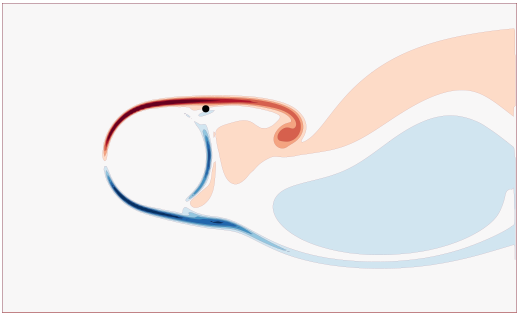
\includegraphics[width=\textwidth]{tex//fig/full_vort.png}
    \end{subfigure}%
    \begin{subfigure}{.5\textwidth}
        \centering
        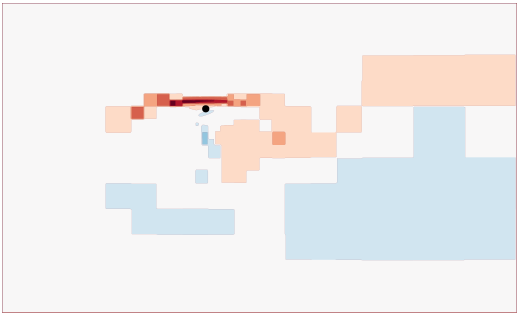
\includegraphics[width=\textwidth]{tex/fig/multilevel_vort.png}
    \end{subfigure}
    \caption{Enter Caption}
    \label{fig:ml_array}
\end{figure}

We propose to replace the standard free-slip or reflection boundary conditions typically applied on the domain's exterior by a \emph{Biot-Savart integral} of the vorticity inside the domain, implicitly assuming the external flow is potential
\begin{equation}\label{eq:Biot}
    {\vec u}({\vec x}) = f(\vec x,\vec\omega) = \int_{\mathcal{V}}K_{n}({\vec x} - \vec{y})\times \vec\omega({\vec y})\text{ d}\vec{y} \quad\quad \forall \vec x\, \in \partial\Omega
\end{equation}
where $K_n$ is the $n$-dimensional Biot-Savart kernel. A Naive evaluation of Equ.~\theequation~ would result in $N^{3/2}$ computation and would erase any benefits brought by a smaller domain. In vortex-particle method, this infinite integral is standard and usually evaluated with \emph{Fast Multipole Method} that allow reducing this cost to $N^{1/2}\log N$ operations. Within our staggered gird arrangement, we use an Algebraic multigrid algorithm to achieve the same reduction in operation.

Substitution of the \emph{Biot-Savart} boundary condition function (Eq.~\ref{eq:Biot}) into the projection scheme shown above results in a slightly modified intermediate velocity field
\begin{align}
    &u^* = \mu_0(u^0+R_{\Delta t})+(1-\mu_0)U_b &\quad\forall\ x\in\Omega\ O(N) \\
    &u^* = f(x_\partial,\nabla\times u^*) &\quad\forall\ x_\partial\in\partial\Omega\ O(N)
\end{align}
where the exterior boundary condition have been computed from the intermediate velocity $u^*$ in the domain. The projection step, however, results in a coupling of the body and the exterior boundary through the pressure field
\begin{align}
  &\nabla\cdot\mu_0\nabla p = \nabla\cdot u^* &\forall\ x\in\Omega O(N)\\
  &u = u^*-\mu_0\nabla p &\quad\forall\ x\in\Omega\ O(N)\\
  &u = f(x_\partial,\nabla\times u)= u^*-f(x_\partial,\nabla\times\mu_0\nabla p) &\quad\forall\ x_\partial\in\partial\Omega\ O(N).
\end{align}
Explicit update of the source term of the Poisson problem during each iteration ensures that the divergence-free constraint is respected
\begin{align}
    &\nabla\cdot\mu_0\nabla p = \nabla\cdot u^*-\nabla\cdot f(x_\partial,\nabla\times\mu_0\nabla p) &\quad\forall\ x\in\Omega, x_\partial\in\partial\Omega\ O(N).
\end{align}

\paragraph{}

\section{Validation Cases}

\subsection{2D validation: Lamb vortex}

The velocity field generated by the Lamb-Chaplygin dipole is obtained from the scalar stream function $\vec{u} = -\vec{e}_z\times \nabla \psi$ given by
\begin{equation}
    \psi = \begin{cases}
    \frac{-2UJ_1(\beta r)}{\beta J_0(\beta R)}, \quad \text{for} \quad r < R,\\
    U\left(\frac{R^2}{r}-r\right), \quad \text{for} \quad r \ge R,    \end{cases}
\end{equation}
%Meleshko, V. V.; Heijst, G. J. F. van (August 1994). "On Chaplygin's investigations of two-dimensional vortex structures in an inviscid fluid". Journal of Fluid Mechanics. 272: 157–182. Bibcode:1994JFM...272..157M. doi:10.1017/S0022112094004428. ISSN 1469-7645. S2CID 123008925.
where $J_0$ and $J_1$ are the zeroth and first Bessel function of the first kind, respectively. $\beta$ is a parameter with the value $\beta=1.2197\pi/R$. The vortex posses an \emph{athmosphere} $\psi(r=R)=0$ that delimits the inside and outside of the vortex.

We use out multilevel method to reconstruct the velocity field generated by the vorticity field obtained by evaluating the vortex equation on the grid. Due to the singularity of the Biot-Savart kernel for $|\vec{x}-\vec{x'}|\to0$, we compute the reconstructed velocity outside the vortex's atmosphere. We investigate the dependency of the reconstructed velocity field to the radius of the multilevel refinement criterion. Results for different kernel radii are shown in Fig.~\ref{fig:lam_error_dist}

\begin{figure}
\begin{subfigure}{.5\textwidth}
  \centering
  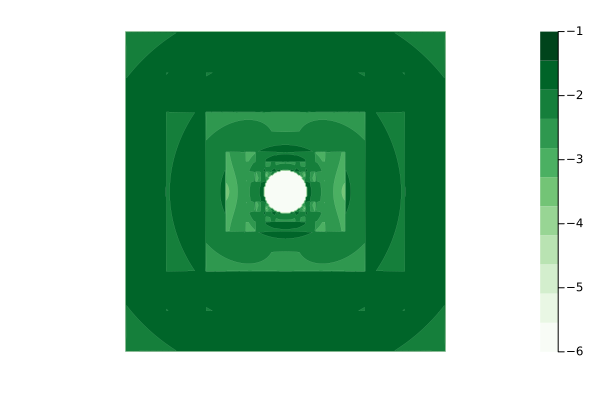
\includegraphics[width=\linewidth]{tex/fig/lamb_dipole_error_dist2.png}
  \caption{}
\end{subfigure}%
\begin{subfigure}{.5\textwidth}
  \centering
  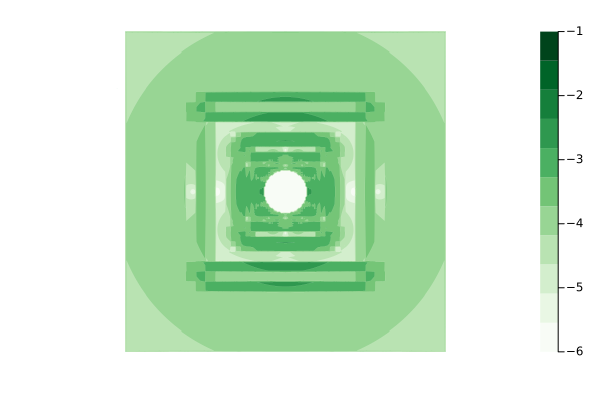
\includegraphics[width=\linewidth]{tex/fig/lamb_dipole_error_dist8.png}
  \caption{}
\end{subfigure}
\begin{subfigure}{.5\textwidth}
  \centering
  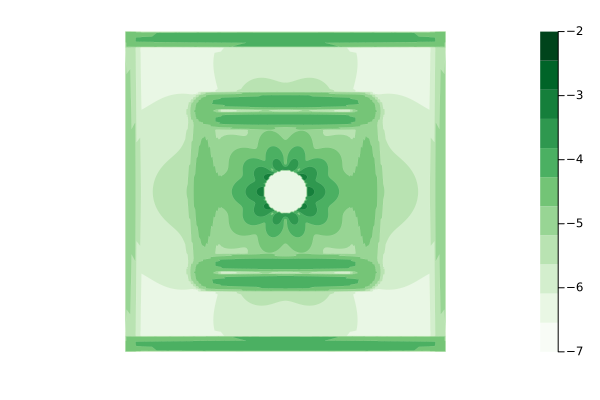
\includegraphics[width=\linewidth]{tex/fig/lamb_dipole_error_dist32.png}
  \caption{}
\end{subfigure}%
\begin{subfigure}{.5\textwidth}
  \centering
  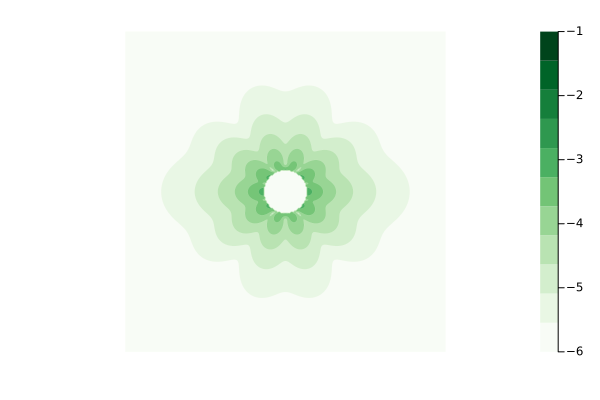
\includegraphics[width=\linewidth]{tex/fig/lamb_dipole_error_dist128.png}
  \caption{}
\end{subfigure}
\caption{$L_2$-norm of the error in reconstructed velocity field outside the atmosphere of the 2D Lamb-Chaplygin vortex for varying (multi-level) kernel size. Error bars are shown in log-scale.}
\label{fig:lam_error_dist}
\end{figure}

The maximum error in the reconstructed velocity field for the Lamb-Chaplygin vortex is shown in Fig.~\ref{fig:error_lamb_2}.

\begin{figure}
    \centering
    \begin{subfigure}{.5\textwidth}
        \centering
        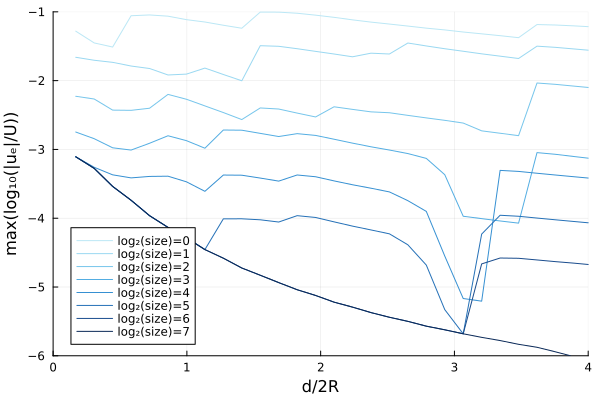
\includegraphics[width=\textwidth]{tex//fig/lamb_dipole_error_dists.png}
    \end{subfigure}%
    \begin{subfigure}{.5\textwidth}
        \centering
        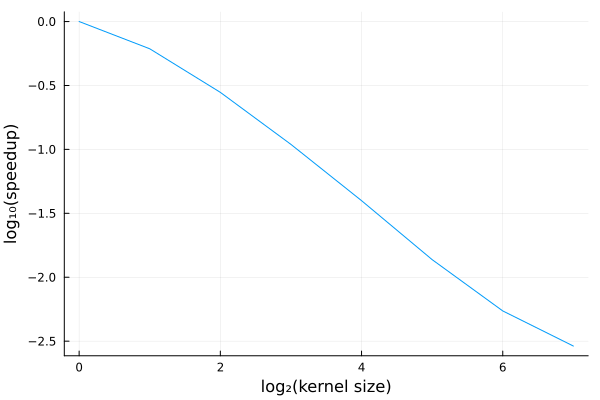
\includegraphics[width=\textwidth]{tex/fig/lamb_dipole_speedup_dists.png}
    \end{subfigure}
    \caption{Enter Caption}
    \label{fig:error_lamb_2}
\end{figure}

\subsection{3D validation: Hill vortex}

Additionally, we validate the reconstruction of the velocity field from a three-dimensionnal vorticity source given by the classical \emph{Hill vortex}, who's radial and tangential velocity components are given by
\begin{align}
    v_r &= \frac{1}{r^2\sin\theta}\frac{\partial\psi}{\partial\theta}, \qquad v_\theta = -\frac{1}{r\sin\theta}\frac{\partial\psi}{\partial r}.
\end{align}
and the stream function 
\begin{equation}
    \psi(r,\theta) = \begin{cases}
    -\frac{3U}{4}\left(1-\frac{r^2}{R^2}\right)r^2sin^2\theta \quad \text{for} \, r \le R,\\
     \,\,\frac{U}{2}\left(1-\frac{r^3}{R^3}\right)r^2sin^2\theta \quad \text{for} \, r > R.
    \end{cases}
\end{equation}

\begin{figure}
    \centering
    \begin{subfigure}{.5\textwidth}
        \centering
        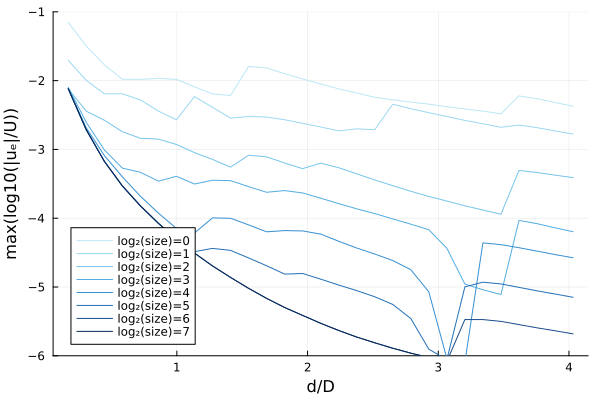
\includegraphics[width=\textwidth]{tex//fig/Hill_error_dists.png}
    \end{subfigure}%
    \begin{subfigure}{.5\textwidth}
        \centering
        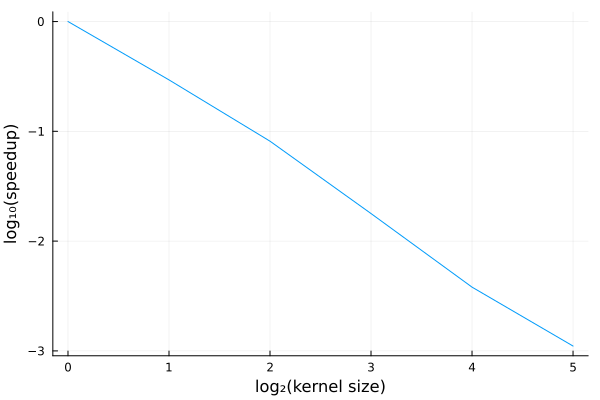
\includegraphics[width=\textwidth]{tex/fig/Hill_speedup_dists.png}
    \end{subfigure}
    \caption{Maximum error in the resonstructed velocity field generated by a 3D \emph{Hill} vortex for various kernel sizes and distances from the vortex core (left). Corresponding speed-up obtained by reducing the kernel size for the multigrid algorithm (right).}
    \label{fig:error_hill_3}
\end{figure}

\subsection{Viscous flow around a cylinder}

\begin{figure}
    \centering
    \begin{subfigure}{.5\textwidth}
        \centering
        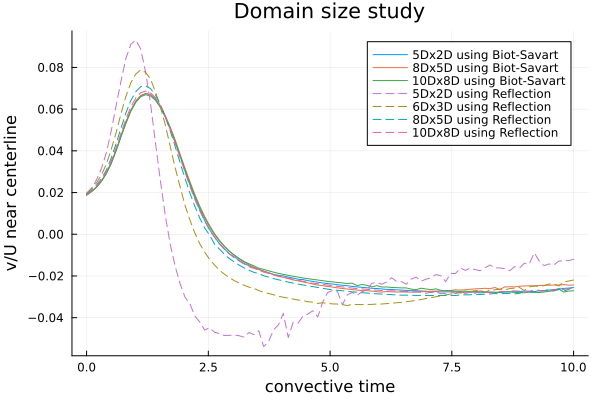
\includegraphics[width=\textwidth]{tex//fig/start.png}
    \end{subfigure}%
    \begin{subfigure}{.5\textwidth}
        \centering
        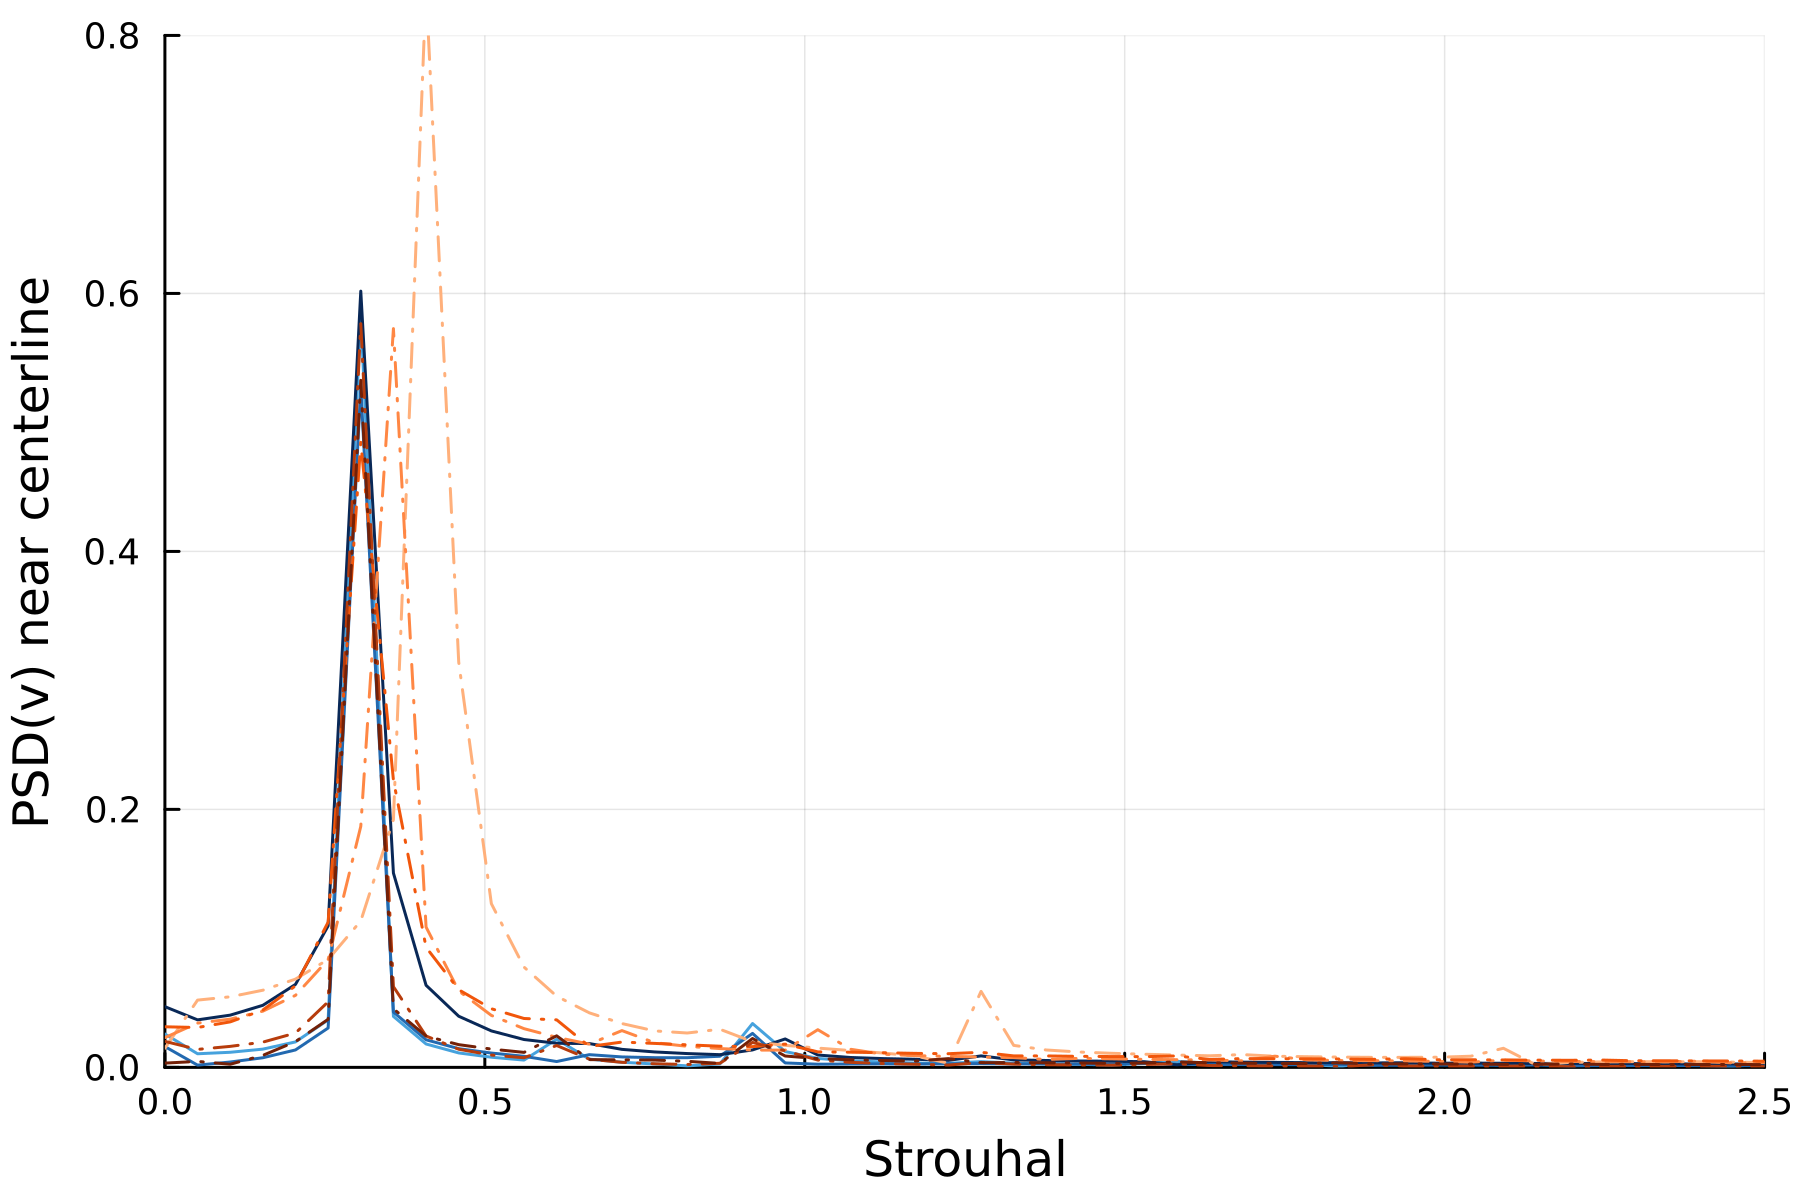
\includegraphics[width=\textwidth]{tex/fig/fft.png}
    \end{subfigure}
    \caption{Enter Caption}
    \label{fig:cylinder_flow}
\end{figure}

\subsection{3D flow around an accelerating disk}

\begin{figure}
    \centering
    \begin{subfigure}{.33\textwidth}
        \centering
        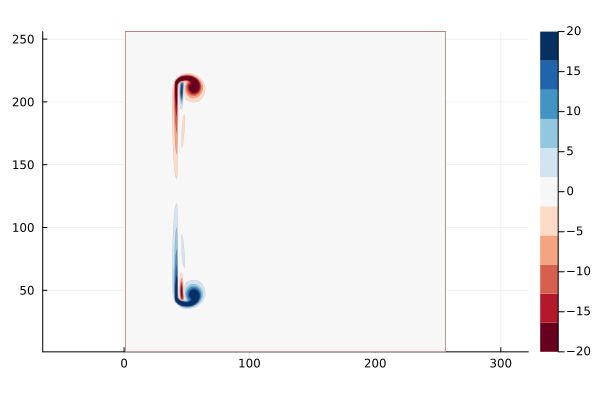
\includegraphics[width=\textwidth]{tex/fig/Disk_reflect_omega_1.png}
    \end{subfigure}%
    \begin{subfigure}{.33\textwidth}
        \centering
        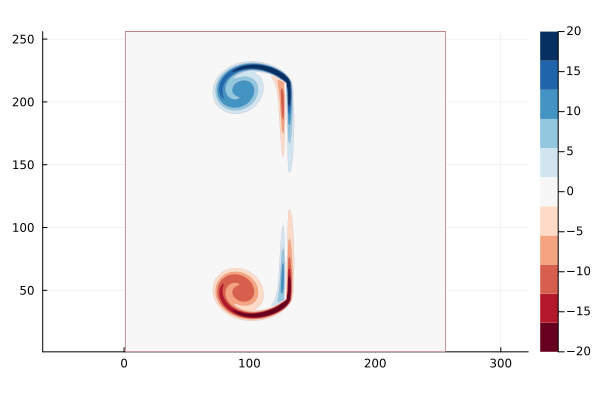
\includegraphics[width=\textwidth]{tex/fig/Disk_reflect_omega_2.png}
    \end{subfigure}%
    \begin{subfigure}{.33\textwidth}
        \centering
        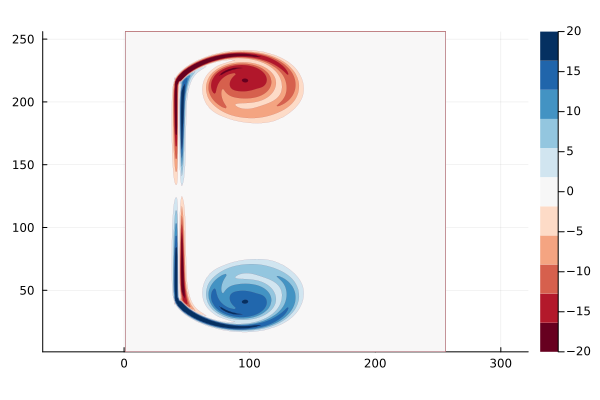
\includegraphics[width=\textwidth]{tex/fig/Disk_reflect_omega_3.png}
    \end{subfigure}
    \caption{Enter Caption}
    \label{fig:disk_flow}
\end{figure}


% \textbf{T. Colonius, H. Ran, A super-grid-scale model for simulating compressible flow on unbounded domains, J. Comput. Phys. 182(2002) 191–212.}

% \textbf{T. Colonius, Modeling artificial boundary conditions for compressible flow, Annu. Rev. Fluid Mech. 36 (2004) 315–345.}

% \textbf{G. Jin, M. Braza, A nonreflecting outlet boundary condition forincompressible unsteady Navier–Stokes calculations, J. Comput.Phys. 107 (1993) 239–253.}

% \textbf{M.A. Ol’shanskii, V.M. Staroverov, On simulation of outflow boundary conditions in finite difference calculations for incompressible fluid, Int. J. Numer. Methods Fluid 33 (2000) 499–534}

% \textbf{R.L. Sani, P.M. Gresho, Resume and remarks on the open boundary condition mini symposium, Int. J. Numer. Methods Fluid 18 (1994)983–1008}

% \textbf{Z.J. Wang, Efficient implementation of the exact numerical farfield boundary condition for Poisson equation on an infinite domain, J.Comput. Phys. 153 (1999) 666–670}
 
\section{Conclusion}
Your conclusion here

\section*{Acknowledgments}
This was supported in part by......

%Bibliography
\bibliographystyle{unsrt}  
\bibliography{references}  


\end{document}